\documentclass[11pt, letterpaper, oneside, twocolumn]{article}
\usepackage{fancyvrb}
\usepackage{float}
\usepackage{subfig}
\usepackage{graphicx,dblfloatfix}
\usepackage[hmargin=1in, vmargin=1in]{geometry}               
\usepackage{enumitem}
\usepackage{tikz}
\usetikzlibrary{arrows,backgrounds,calc,fit,mindmap,positioning,trees,shapes}

% \usepackage{fullpage}
% \usepackage{xunicode,xltxtra,url,parskip} 	%other packages for formatting

% \addtolength{\topmargin}{-.5in}
% \addtolength{\bottommargin}{-.875in}
% \addtolength{\textheight}{1.75in}

\setitemize{noitemsep,topsep=0pt,parsep=0pt,partopsep=0pt}
\DefineVerbatimEnvironment{code}{Verbatim}{fontsize=\small}

\newcommand{\tab}{\hspace*{2em}}
\floatstyle{plain}
\restylefloat{figure}
\begin{document}
\title{Yippee: Web Search for the New Millenium}
\author{	TJ Du, Chris Imbriano, Margarita Miranda, Nikos Vasilakis\\
	\{tdu2, imbriano, mmiran, nvas\}@seas.upenn.edu}
\date{May 8, 2012}

\maketitle

\begin{figure*}[ht]
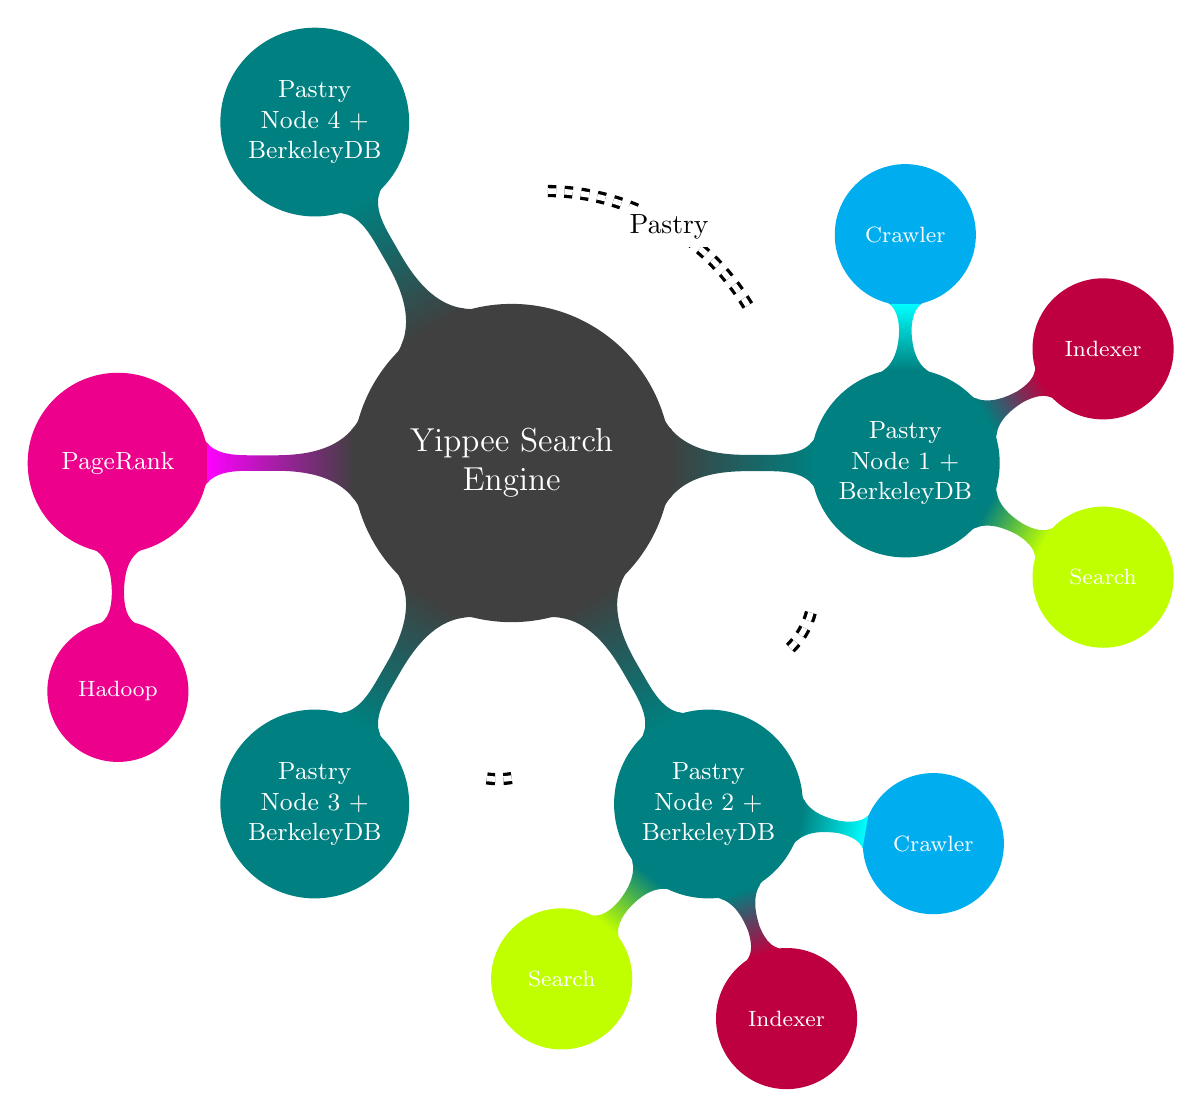
\begin{tikzpicture}
  \path[mindmap,concept color=darkgray,text=white]
    node[concept] {Yippee Search Engine}
    [clockwise from=0]
    child[concept color=teal!] {
      node[concept] {Pastry Node 1 + BerkeleyDB}
      [clockwise from=90]
      child [concept color=cyan!] { node[concept] (c1) {Crawler} }
      child [concept color=purple!]  { node[concept] (i1) {Indexer} }
      child [concept color=lime!] { node[concept] (s1) {Search} }
    }  
    child[concept color=teal!] {
      node[concept] {Pastry Node 2 + BerkeleyDB}
      [clockwise from=-10]
      child [concept color=cyan!] { node[concept] (c2) {Crawler} }
      child [concept color=purple!] { node[concept] (i2) {Indexer} }
      child [concept color=lime!] { node[concept] (s2) {Search} }
    }
    child[concept color=teal!] { node[concept] {Pastry Node 3 + BerkeleyDB} }
    child[concept color=magenta!] {
      node[concept] {PageRank}
      [clockwise from=-90]
      child { node[concept] {Hadoop} }
    }
    child[concept color=teal!] { node[concept] {Pastry Node 4 + BerkeleyDB} };

    \begin{pgfonlayer}{background}
        % \draw [circle connection bar ] (i1) edge [color=violet!50!] (i2);
        % \draw[-to,shorten >=10pt,gray] (c1) -- (c2);
        \draw[very thick, dashed, double distance=2pt] (3,2) arc (31:90:3cm);
        \draw[very thick, dashed, double distance=2pt] (3.8,-1.9) arc (-15:-50:1cm);
        \draw[very thick, dashed, double distance=2pt] (0,-4.0) arc (-80:-100:1cm);
        %\node[anchor=north,text width=10cm,inner sep=.05cm,align=center,fill=white] at (2,2) {Pastry}; text width=3cm,
        \node[fill=white, inner sep=0.1cm, text centered] at (2,3) {Pastry};
    \end{pgfonlayer}
\end{tikzpicture}
  \caption{Yippee's fully distributed architecture. Nodes communicate
  via FreePastry}
\end{figure*}

\section{ Introduction }

To say the world wide web is enormous would be an understatement.  
In the last month (March 2012),  Google's index size was estimated to be between forty-five and fifty-five billion pages.\cite{websize}
The task of presenting a web user with relevant pages according to keyword search has proven to be a difficult one, as many of the commercial search engines during the dawn of the web were unable to return their own site for a search for their site's name.\cite{google} 
Google has shown that besides the load speed of the results, page relevance is just as critical a metric of an effective search engine. 

Yippee is a distributed search engine designed to provide fast, relevant results to keyword queries via the web.  

\section{Project Approach}
\label{sec:approach}

The Yippee Search Engine is a distributed application comprised of 4 main components: a web crawler to recursively download pages from the web, an indexer to index crawled web pages, our simplistic implementation of Google's PageRank algorithm \cite{pagerank}, and a search module to retrieve documents based on user-provided keywords.  
The crawler, indexer and search components are distributed via the FreePastry peer-to-peer substrate, while the PageRank components is centralized.  All parts of the project are deployed to Amazon Elastic Cloud Computing (EC2) instances.  

The architecture of the Yippee is shown in figure \textbf{Update this graph} 1 \textbf{make this number a reference since there will be more figures this time}.


Section \ref{sec:component} will describe each component and its relevant design decision.
Section \ref{sec:evaluation} will present evaluations for some of the design decisions. \textbf{rephrase}

\textbf{These paragraphs probably belong in component discussion}




\label{sec:SOAR} %software architecture
\begin{figure}[!b]
  \centering
  \includegraphics[scale=0.45]{figures/yippee_map.pdf}
  \caption{Software Architecture.}
\end{figure}



\section{Component Discussion}
\label{sec:component}



\subsection{Infrastructure and Software Engineering}

* Build process - ant, EntryPoint, Configuration
* Testing - JUnit
* Persistent Storage - BerkeleyDB
* Distributed Application - FreePastry 

\subsection{Crawler}

The Yippee crawler is a multithreaded distributed crawler based on the design of the Mercator crawler\cite{mercator}. 
Each of the Yippee node is responsible for a subset of the web as determined by FreePastry key-based routing keyed on the host of each url discovered.
Mercator uses various implementations of the URLFrontier to fine tune the crawlers performance and politeness.
For this reason, we made our frontier pluggable via a factory pattern and interface.
This allowed us to easily test frontiers with varying degrees of politeness and performance.

One criticism of the Mercator design\cite{ubi,para} is the centralized nature of the URLFrontier. 

\textbf{Needs to be edited}
Our crawler follows the Mercator design; however, since the design is
criticized for its centralized URLFrontier , we made this
component pluggable. That  way, we can easily plug in different implementations 
and analyze the  performance. Raw content  is  written to a persistent, shared queue  
between the crawler and  the indexer, enabling
asynchronous indexing and page-rank.

\subsection{Indexer}

\textbf{Needs to be edited}
The Indexer will parse the raw content of the url pages that the Crawler crawls and perform two main functions.
First, it will extract links for the URL Resolver that will convert those urls into DocIds.
This information will get fed into PageRank.
Secondly, the Indexer will take the list of all the words in the document and turn them into hit lists containing the DocID, the wordID taken from the lexicon, position in document, and any other useful document specific information for that word. 
Those hit lists will be placed into barrels organized by wordID and the barrels will eventually get sorted to the inverted index which is necessary for the Search Engine.

\subsection{PageRank}

The PageRank component of Yippee is the only centralized part of the system.
It performs a calculation based-on \[Brin, Page 1999\]\cite{pagerank} to determine the relative importance of each page in the index.
The PageRank calculation is an iterative MapReduce running on a single-node Hadoop cluster after retrieving, from each Yippee node, a log of links found during the indexing process.
We decided that PageRank should not be a distributed component for the following reasons. 
First, PageRank is a calcualtion relevant only when doing searches and since the Yippee Search Engine would only be in deployment for a short period of time, it was unlikely that we would have crawled 
There was a decision as to whether or not PageRank should be a distributed component Yippee. 
Some of the factors in this decision were how frequently the rankings would need to be updated and how long the Yippee Search Engine would be in production.

however, given that the lifetime of the working project would be short, repeated calculations of PageRank would be unnecessary, as values would only change 

\subsection{Search}
\textbf{Needs to be edited}
The final piece of Yippee involves presenting the user with highly relevant pages given a provided keyword.
Once a keyword search is received, a heuristic aggregator will calculate highly relevant documents given queries to the indexed data.
The precise details of the heuristic aggregator have yet to be determined, but the main idea is to shrink the pool of possible results as much as possible using metrics like TF/IDF, word count and position, etc.
For these relevant pages, the PageRank score will be taking into account to calculate a final ordering of results to be returned.

\section{Evaluation}
\label{sec:evaluation}

\section{Future Work}
\label{sec:future}

\begin{enumerate}
\item Spell-check
\item Ability to add more nodes/remove nodes on the fly
\item User feedback on query results
\end{enumerate}


\textbf{edit}
If we have additional time, we will implement a spell-check and AJAX support for users to give feedback on query results.


\section{Conclusion}
\label{sec:conculsion}

\section{ Division of Labor }
\label{sec:labor}

While each member of the group is ultimately responsible for monitoring progress and completion of one of the four components described in Section 2, no individual is tasked with its implementation.
Instead, the group collectively determines the high level architecture and component interfaces, then a pair of members implements their assigned component.
The other two group members will write black box tests of the agreed upon interface without inspecting the source code such that their tests are unbiased towards any particular implementation decision.
The sign-off responsibility is divided as follows: Crawler - Nikos, Indexer - Margarita, PageRank - Chris, Search Engine and Web UI - TJ.

For the first milestone, Chris and Nikos will work on the Crawler and the preliminary components of FreePastry, and TJ and Margarita will work on the Indexer.
The same approach will be used for PageRank and User Interface but the team members may be shuffled.

\begin{thebibliography}{9}

  \bibitem{websize} WorldWideWebSize.com, 11 Apr 2012 $\langle$http://www.worldwidewebsize.com$\rangle$
  \bibitem{google} Sergey Brin and Lawrence Page \emph{The Anatomy of a Large-Scale Hypertextual Web Search Engine}, Stanford University, 1999
  \bibitem{pagerank} Sergey Brin and  Lawrence Page and Rajeev Motwani and Terry Winograd \emph{The PageRank Citation Ranking: Bringing Order to the Web}, Stanford InfoLab, 1999
  \bibitem{mercator} Allan Heydon and Marc Najork, \emph{Mercator: A scalable, extensible web crawler}, Compaq Systems Research Center, September 26, 2001
  \bibitem{ubi} Paolo Boldi, Bruno Codenotti, Massimo Santini, Sebastiano Vigna, \emph{UbiCrawler: a scalable fully distributed Web crawler}, Software: Practice and Experience 34 (2004), 711-726.
  \bibitem{para} Junghoo Cho, H\'{e}ctor Garcia-Molina, \emph{Parallel crawlers}, Proc. of the 11th International Conference on World Wide Web, 2002.


\end{thebibliography}

\end{document}
